% Freerange VHDL
% Authors: Bryan Mealy, Fabrizio Tappero
% Date: May, 2011
%
% (C) 2011 B. Mealy, F. Tappero
%
% !TEX root = freerange_vhdl_master.tex
%
\chapter{Data Objects}

Many of the concepts presented so far have been implicitly presented in the context of example problems. In this way, you have probably been able to generate quality VHDL code but were constrained to use the VHDL style presented in these examples. In this section, we will present some of the underlying details and theories that surround VHDL as a backdoor approach for presenting tools that will allow you to use VHDL for describing the behaviour of more complex digital circuits.

In order to move into more sophisticated VHDL, a good place to start is with the definition of VHDL objects (e.g. data types). An object is an item in VHDL that has both a name (associated identifier) and a specific type. There are four types of objects and many different data types in VHDL. Up to this point, we have only used \texttt{signal} data objects and \texttt{std\_logic} data types. Two new data objects and several new data types are introduced and discussed in this section.

\section{Types of Data Objects}
There are four types of data objects in VHDL: signals, variables, constants, and files. One of the purposes of this section is to present some background information regarding variables which will be used later in this tutorial. The idea of constants will also be briefly mentioned since they are generally straight-forward to understand and use once the concepts of signals and variables are understood. File data objects are not discussed in this tutorial. 

Mind that VHDL is vast programming language that goes well beyond the VHDL code that is used to program an FPGA or a CPLD. In fact the actual VHDL that can be translate into an FPGA/CPLD bit-stream is called RTL VHDL and represent only a small subset of what is included in the current VHDL standard. The file  data objects is an example of data object that can not be implemented in a silicon device.

Just as side note, it is interesting to point out that it is also possible to compile VHDL code into an executable file that can be executed, generally for simulation purposes, with any general purpose Intel PC. For more details refer to the open-source work of T. Gingold available at \url{http://ghdl.free.fr}.

\section{Data Object Declarations}

The first thing to note about data objects is the similarity in their declarations. The forms for the three data objects we will be discussing are listed in Table \ref{vhdl_data_objs}. For each of these declarations, the bold-face font is used to indicate VHDL keywords. The form for the signal object should seem familiar since we have used it extensively up to this point.

\begin{table}[!h]
\centering
\footnotesize\textsf{\begin{tabular}{ l l }
\hline
\rowcolor{gray} \textbf{VHDL data object} & \textbf{Declaration form}\\
\hline
\rowcolor{light-gray} Signal & \texttt{{\bf signal} sig\_name : sig\_type := initial\_value;} \\
\hline
Variable & \texttt{{\bf variable} var\_name : var\_type := initial\_value;} \\
\hline
\rowcolor{light-gray} Constant & \texttt{{\bf constant} const\_name : const\_type := initial\_value;} \\
\hline
\end{tabular}}
\caption{Data object declaration forms.}
\label{vhdl_data_objs}
\end{table}

Note that each of the data objects can optionally be assigned initial values to. As you know, signal declarations do not usually include initial values as opposed to constants which generally do. Example declarations for these three flavors of data objects are provided in Table \ref{vhdl_data_objs_ex}. These examples include several new data types which will be discussed in the next section. 

\begin{table}[!h]
\centering
\footnotesize\textsf{\begin{tabular}{ l l }
\hline
\rowcolor{gray} \textbf{Data object} & \textbf{Declaration form}\\
\hline
Signal & \texttt{{\bf signal} sig\_var1 : std\_logic := '0';} \\
& \texttt{{\bf signal} tmp\_bus : std\_logic\_vector(3 downto 0) := "0011";} \\
& \texttt{{\bf signal} tmp\_int : integer range -128 to 127 := 0;}  \\
& \texttt{{\bf signal} my\_int : integer;}\\
\hline
Variable &\texttt{{\bf variable} my\_var1, my\_var2 : std\_logic;} \\
&\texttt{{\bf variable} index\_a : integer range (0 to 255) := 0;} \\ 
&\texttt{{\bf variable} index\_b : integer := -34;} \\
\hline
Constant & \texttt{{\bf constant} sel\_val : std\_logic\_vector(2 downto 0) := "001";} \\
&\texttt{{\bf constant} max\_cnt : integer := 12;} \\
\hline
\end{tabular}}
\caption{Example declarations for signal, variable, and constant data objects.}
\label{vhdl_data_objs_ex}
\end{table}

\section{Variables and the Assignment Operator ``\texttt{:=}''}
Although variables are similar to signals, variables are not as functional for the several reasons mentioned in this section. Variables can only be declared and used inside of processes, functions, and procedures (functions and procedures will not be discussed here). Implied in this statement is the sequential nature of variable assignment statements in that all statements appearing in the body of a process are sequential. One of the early mistakes made by VHDL programmers is attempting to use variables outside of processes.

The signal assignment operator, $<=$, was used to transfer the value of one signal to another with dealing with signal data objects. When working with variables, the assignment operator $:=$ is used to transfer the value of one variable data object to another. As you can see from Table \ref{vhdl_data_objs_ex}, the assignment operator is overloaded which allows it to be used to assign initial values to the three listed forms of data objects.

\section{Signals vs. Variables}
The use of signals and variables can be somewhat confusing because of their similarities. Generally speaking, a signal can be thought of as representing a wire or some type of physical connection in a design. Signals thus represent a mean to interface VHDL modules which includes connections to the outside world. In terms of circuit simulation, signals can be scheduled to take on multiple values at specific times in the simulation. The specifics of simulating circuits using VHDL are not covered here so the last statement may not carry much meaning to you. The important difference here is that events can be scheduled for signals while for variables, they cannot. The assignment of variables is considered to happen immediately and cannot have a list of scheduled events.

With relatively simple circuits, signal objects are generally sufficient. As your digital designs become more complex, there is a greater chance that you will need more control of your models than signals alone can provide. The main characteristic of signals that leave them somewhat limited in complex designs is when and how they are scheduled. More specifically, assignments made to signals inside a process are actually only scheduled when the same process is completed. The actual assignment is not made until after the process terminates. This is why multiple signal assignments can be made to the same signal during the execution of a process without generating any type of synthesis error. In the case of multiple signal assignments inside the process, only the most recent assignment to the signal during process execution is assigned. The important thing here is that the signal assignment is not made until after the process terminates. The potential problem that you might face is that the new result (the new value assigned to the signal) is not available to use inside the process. 

Variable assignment within processes is different. When a variable is assigned a value inside of a process, the assignment is immediate and the newly assigned value can be used immediately inside of the process. In other words, the variable assignment is not scheduled as it was for the signal. This is a giant difference and has massive ramifications in both the circuit simulation and synthesis realm. 

Variables cannot always be modelled as wires in a circuit. They also have no concept of memory since they cannot store events. With all this in mind, you may wonder the appropriate place to use variables. The answer is variables should only be used as iteration counters in loops or as temporary values when executing an algorithm that performs some type of calculation. It is possible to use variables outside of these areas, but it should be avoided.

\section{Data Types}
Not only does VHDL have many defined data types but VHDL also allows you to define your own types. Here however we will only deal with few of the most widely used types. In this section, the types that have already been discussed are listed and a few more popular and useful types are introduces. 

\section{Commonly Used Types}

The types already introduced in previous chapters as well as two new types are listed in Table \ref{vhdl_data_types}. The \texttt{std\_logic} and \texttt{std\_logic\_vector} types have been extensively used so far. These types are more complex then has been previously stated and will be discussed further in this chapter. The \texttt{enumerated} type was used during the previous discussion of finite states machines. The \texttt{integer} type was cryptically mentioned before but it will be discussed further along with the \texttt{boolean} type in this chapter. 

\begin{table}[!h]
\centering
\footnotesize\textsf{\begin{tabular}{ l l l}
\hline
\rowcolor{gray} \textbf{Type} & \textbf{Example} & \textbf{Usage} \\
\hline
\rowcolor{light-gray} std\_logic & \texttt{{\bf signal} my\_sig : {\bf std\_logic};} & all examples \\
\hline
std\_logic\_vectors & \texttt{{\bf signal} busA : {\bf std\_logic\_vector}(3 downto 0)}; & all examples \\
\hline
\rowcolor{light-gray} enumerated &  \texttt{{\bf type} state\_type {\bf is} (ST0,ST1,ST2,ST3);} & Example 18\\
\hline
boolean & \texttt{{\bf variable} my\_test : {\bf boolean} := {\bf false};} & None \\
\hline
\rowcolor{light-gray} integer & \texttt{{\bf signal} iter\_cnt : {\bf integer} := 0;}  & Example 26 \\
\hline
\end{tabular}}
\caption{Some popular data types already introduced in previous chapters.}
\label{vhdl_data_types}
\end{table}

\section{Integer Types}
The use of integer types aids in the design of algorithmic-type VHDL code. This type of coding allows VHDL to describe the behaviour of complex digital circuits. As you progress in your digital studies, you will soon find yourself in need of more complex descriptive VHDL tools. Data types such as integers partially fills that desire. This section briefly looks at integer types as well as the definition of user specified integer types.

The range of the integer type is [-2,147,483,647 to 2,147,483,647]. These numbers should seem familiar since they represent the standard 32-bit range for a signed number: (-231 to +231). Other types similar to integers includes natural and positive types. These types are basically integers with shifted ranges. For example, the natural and positive types range from 0 and 1 to the full 32-bit range, respectively. Examples of integer declarations are shown in the following listing.
\vspace{8pt}
\begin{lstlisting}

-- integer declarations
signal my_int : integer range 0 to 255 := 0;
variable max_range : integer := 255;
constant start_addr : integer:= 512;
\end{lstlisting}

Although it could be possible to use only basic integer declarations in your code, VHDL allows you to define you own integer types with their own personalised range constraints. These special types should be used where possible to make you code more readable. These type definitions use the \texttt{type} \texttt{range} construct and the \texttt{to} or the \texttt{downto} keywords for the definition. Some examples of integer-type declarations are provided in the following listing.
\vspace{8pt}
\begin{lstlisting}

-- integer type declarations
type scores  is range 0 to 100; 
type years   is range -3000 to 3000; 
type apples  is range 0 to 15; 
type oranges is range 0 to 15; 
\end{lstlisting}

Although each of the types listed in the previous listing are basically integers, they are still considered different types and cannot be assigned to each other. In addition to this, any worthy VHDL synthesizer will do range checks on your integer types. In the context of the definitions previously presented, each of the statements in in the following listing is illegal. 
\vspace{8pt}
\begin{lstlisting}

-- Illegal assignment statements
signal score1    : scores  := 100;  
signal my_apple  : apples  := 0; 
signal my_orange : oranges := 0; 

my_apple <= my_orange;  -- different types
my_orange <= 24;        -- out of range
my_score <= 110;        -- out of range
\end{lstlisting}

\section{The \texttt{std\_logic} Type}
For the representation of digital signals, so far in this book, we have use the \texttt{std\_logic} type. However, one of the data types not used or not listed in this book is the \texttt{bit} type. This type can take on only the values of '1' or '0' only. While this set of values seems appropriate for designing digital circuits, it is actually somewhat limited. Due to its versatility and a more complete range of possible values, the \texttt{std\_logic} type is preferred over \texttt{bit} types. The \texttt{std\_logic} type is officially defined in the VHDL STANDARD package and provides a common standard that can be used by all VHDL programmers.

The \texttt{std\_logic} type is officially defined as an \texttt{enumerated} type. Two of the possible enumerations of course include '1' and '0'. The actual definition is shown in the listing \ref{ulogic_type}. As you can see, this definition lists \texttt{std\_ulogic} as opposed to the \texttt{std\_logic} you are used to. The \texttt{std\_logic} type is a \textit{resolved} version of the \texttt{std\_ulogic} type. The exact meaning of resolution is beyond the scope of this book and can be safely overlooked. 

\begin{lstlisting}[label=ulogic_type, caption=Declaration of the \texttt{std\_ulogic} enumerated type.]
type std_ulogic is ( 'U', -- uninitialised 
                     'X', -- forcing unknown
                     '0', -- forcing 0
                     '1', -- forcing 1
                     'Z', -- high impedance
                     'W', -- weak unknown
                     'L', -- weak 0
                     'H', -- weak 1
                     '-'  -- unspecified (do not care) 
                   );
\end{lstlisting}

The \texttt{std\_ulogic} type uses the VHDL character type in its definition. Although there are nine values in the definition shown in listing \ref{ulogic_type}, this book only deals with '0', '1', 'Z', and '-'. The 'Z' if generally used when dealing with bus structures. This allows a signal or set of signals (a bus) to have the possibility of being driven by multiple sources without the need to generate resolution functions. When a signal is driven to its high impedance state, the signal is not driven from that source and is effectively removed from the circuit. And finally, since the characters used in the \texttt{std\_ulogic} type are part of the definition, they must be used as listed. Mind the the use of lower-case letters will generate an error. 





\begin{leftbar}
\begin{minipage}[t]{0.52\textwidth}
\vspace{10pt}
\noindent
\textbf{EXAMPLE 26.}
Design a clock divider circuit that reduces the frequency of the input signal by a factor of 64. The circuit has two inputs as shown in the diagram. The div\_en input allows the clk signal to be divided when asserted and the sclk output will exhibit a frequency 1/64 that of the clk signal. When div\_en is not asserted, the sclk output remains low. Frequency division resets when the div\_en signal is reasserted.
\end{minipage}
\begin{minipage}[t]{0.47\textwidth}
\vspace{0pt}\raggedright
    \centering
	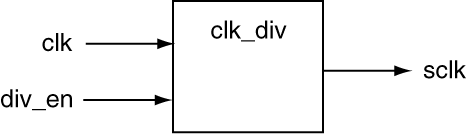
\includegraphics[width=5.2cm]{do/ex26.png}
\end{minipage}
\end{leftbar}

\noindent
\textbf{SOLUTION.} As usual for more complex concepts and circuits, there are a seemingly infinite number of solutions. A solution that uses several of the concepts discussed in this section is presented in listing \ref{ex26_code}. Some of the more important issues in this solution are listed below.

\begin{my_list}
\item The type declaration for my\_count appears in the architecture body before the \texttt{begin} statement. 

\item A constant is used for the max\_count variable. This allows for quick adjustments in the clock frequency. In this example, this concept is somewhat trivial because the max\_count variable is used only once.  

\item The variable is declared inside of the process, after the process \texttt{begin} line.
\end{my_list}

\begin{lstlisting}[label=ex26_code, caption=Solution to EXAMPLE 26.]
entity clk_div is
    Port (    clk : in std_logic;
           div_en : in std_logic;
             sclk : out std_logic);
end clk_div;

architecture my_clk_div of clk_div is

   type my_count is range 0 to 100;        -- user-defined type
   constant max_count : my_count := 63;    -- user-defined constant
   signal tmp_sclk : std_logic;            -- intermediate signal for clock
   
begin
   my_div: process (clk, div_en)   
      variable div_count : my_count := 0; 

   begin
      if (rising_edge(clk)) then            -- look for clock edge
         if (div_en = '1') then             -- divider enabled
            if (div_count = max_count) then 
               tmp_sclk <= not tmp_sclk;    -- toggle output
               div_count := 0;              -- reset count
            else
               div_count := div_count + 1; 
            end if; 
         else                       -- divider disabled
            div_count := 0;         -- reset count 
            tmp_sclk <= '0';        -- turn off output
         end if; 
      end if; 
   end process my_div; 

   s_clk <= tmp_sclk;   -- assign to output
end my_clk_div;
\end{lstlisting}





